% Options for packages loaded elsewhere
\PassOptionsToPackage{unicode}{hyperref}
\PassOptionsToPackage{hyphens}{url}
%
\documentclass[
  openany]{book}
\usepackage{lmodern}
\usepackage{amssymb,amsmath}
\usepackage{ifxetex,ifluatex}
\ifnum 0\ifxetex 1\fi\ifluatex 1\fi=0 % if pdftex
  \usepackage[T1]{fontenc}
  \usepackage[utf8]{inputenc}
  \usepackage{textcomp} % provide euro and other symbols
\else % if luatex or xetex
  \usepackage{unicode-math}
  \defaultfontfeatures{Scale=MatchLowercase}
  \defaultfontfeatures[\rmfamily]{Ligatures=TeX,Scale=1}
\fi
% Use upquote if available, for straight quotes in verbatim environments
\IfFileExists{upquote.sty}{\usepackage{upquote}}{}
\IfFileExists{microtype.sty}{% use microtype if available
  \usepackage[]{microtype}
  \UseMicrotypeSet[protrusion]{basicmath} % disable protrusion for tt fonts
}{}
\makeatletter
\@ifundefined{KOMAClassName}{% if non-KOMA class
  \IfFileExists{parskip.sty}{%
    \usepackage{parskip}
  }{% else
    \setlength{\parindent}{0pt}
    \setlength{\parskip}{6pt plus 2pt minus 1pt}}
}{% if KOMA class
  \KOMAoptions{parskip=half}}
\makeatother
\usepackage{xcolor}
\IfFileExists{xurl.sty}{\usepackage{xurl}}{} % add URL line breaks if available
\IfFileExists{bookmark.sty}{\usepackage{bookmark}}{\usepackage{hyperref}}
\hypersetup{
  pdftitle={A minibook collection of AH Annotations},
  pdfauthor={Cassie Tanks},
  hidelinks,
  pdfcreator={LaTeX via pandoc}}
\urlstyle{same} % disable monospaced font for URLs
\usepackage{longtable,booktabs}
% Correct order of tables after \paragraph or \subparagraph
\usepackage{etoolbox}
\makeatletter
\patchcmd\longtable{\par}{\if@noskipsec\mbox{}\fi\par}{}{}
\makeatother
% Allow footnotes in longtable head/foot
\IfFileExists{footnotehyper.sty}{\usepackage{footnotehyper}}{\usepackage{footnote}}
\makesavenoteenv{longtable}
\usepackage{graphicx,grffile}
\makeatletter
\def\maxwidth{\ifdim\Gin@nat@width>\linewidth\linewidth\else\Gin@nat@width\fi}
\def\maxheight{\ifdim\Gin@nat@height>\textheight\textheight\else\Gin@nat@height\fi}
\makeatother
% Scale images if necessary, so that they will not overflow the page
% margins by default, and it is still possible to overwrite the defaults
% using explicit options in \includegraphics[width, height, ...]{}
\setkeys{Gin}{width=\maxwidth,height=\maxheight,keepaspectratio}
% Set default figure placement to htbp
\makeatletter
\def\fps@figure{htbp}
\makeatother
\setlength{\emergencystretch}{3em} % prevent overfull lines
\providecommand{\tightlist}{%
  \setlength{\itemsep}{0pt}\setlength{\parskip}{0pt}}
\setcounter{secnumdepth}{5}

\title{A minibook collection of AH Annotations}
\author{Cassie Tanks}
\date{}

\begin{document}
\maketitle

{
\setcounter{tocdepth}{1}
\tableofcontents
}
\hypertarget{this-is-an-example-of-how-i-can-create-an-open-text-book-or-other-collection-of-works.}{%
\chapter{This is an example of how I can create an open text book or other collection of works.}\label{this-is-an-example-of-how-i-can-create-an-open-text-book-or-other-collection-of-works.}}

\hypertarget{introduction}{%
\chapter{Introduction}\label{introduction}}

This is where I will introduce the work I have been doing as an graduate research assistant for \emph{Apartheid Heritage(s)}. Of course, I will need to introduce \emph{my} trusty research assistant, Byrone ``Buster'' Bluth.
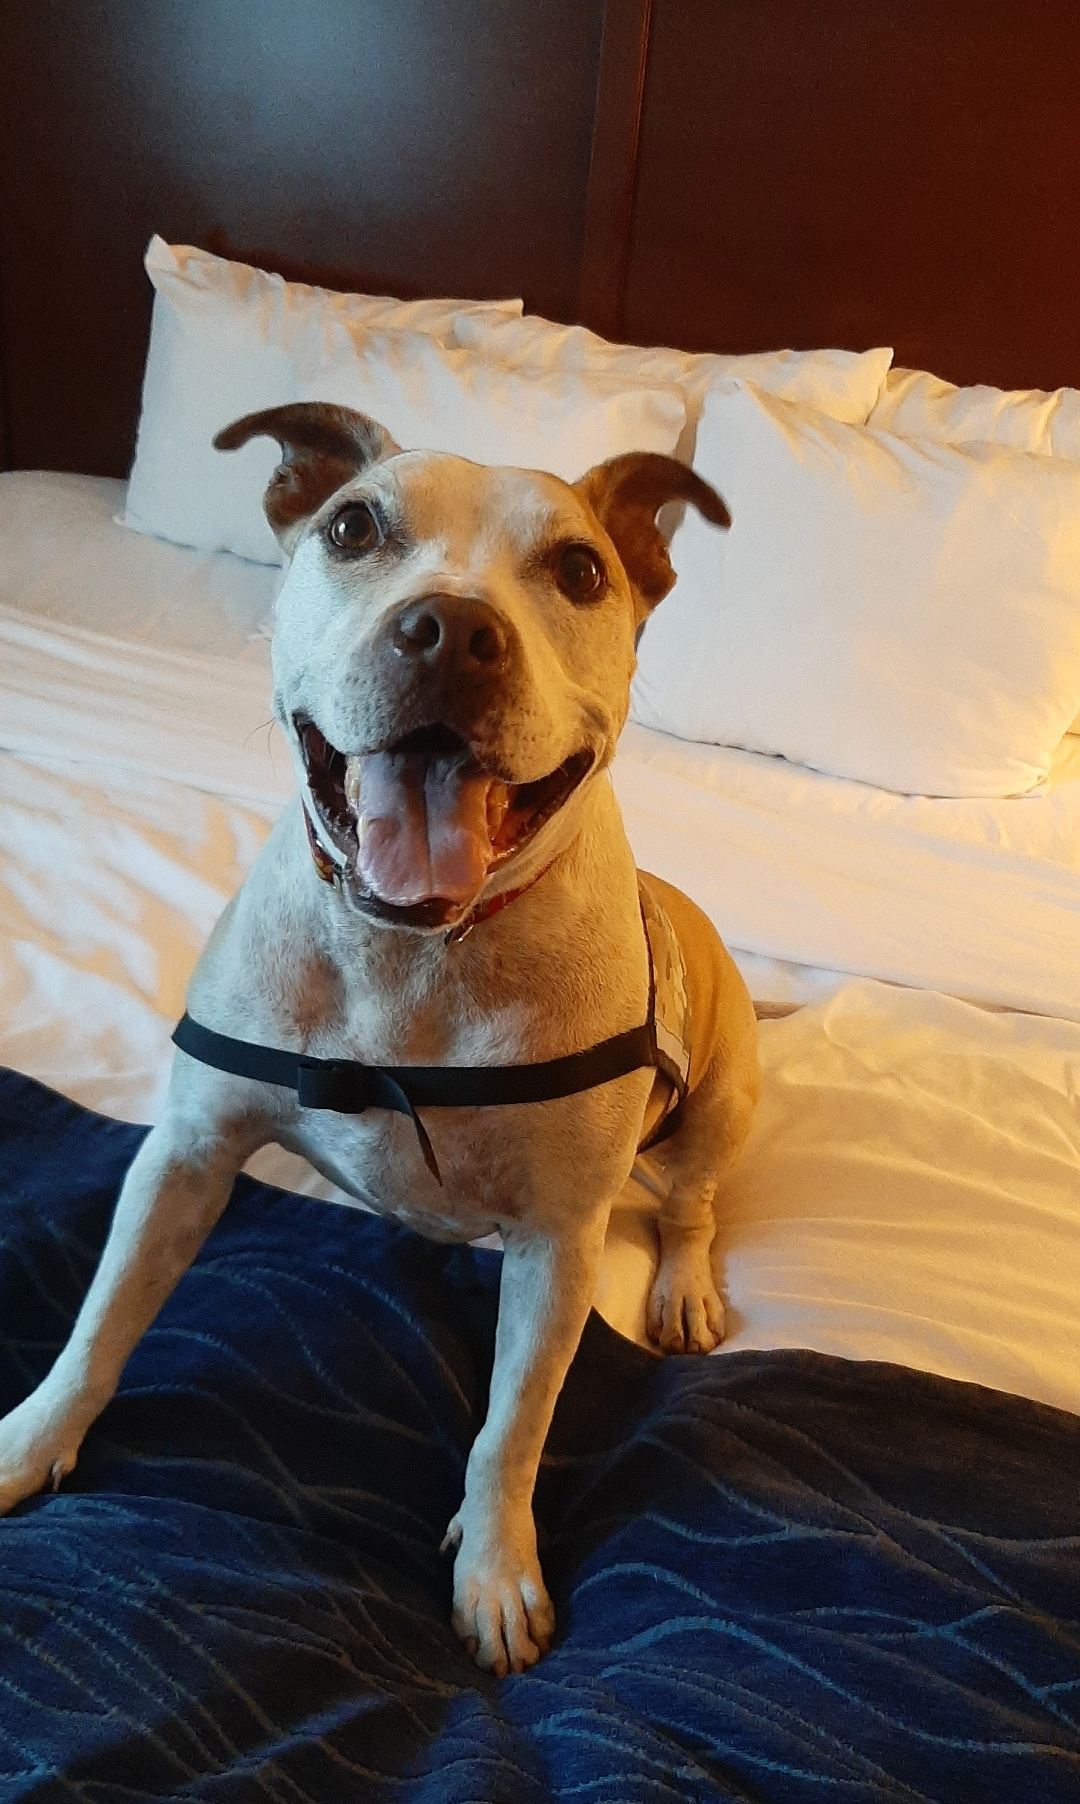
\includegraphics{202006_Buster_Hotel.jpg}

Primarily, I will discuss my role in rethinking and creating annotations for a digital humanities project that examines contested spacial history by exploring specific places in a 3D model.

I will include block quotes to emphasize the methodology of the work and the many conversations I have had with Dr.~Nieves.

\begin{quote}
Block quote that shows off the research that has been done. So much research will be exemplified here and readers will be \emph{impressed}.
\end{quote}

\#Assemblages
\#\#\#\# \emph{Organization of the Annotations}

This is just practice. There is no real content in this chapter (yet).
Now I will add an ordered list.
1. Assemblage 1
2. Assemblage 2
3. Assemblage 3
4. Assemblage 4

\hypertarget{assemblage-1}{%
\subparagraph{Assemblage 1}\label{assemblage-1}}

Here is where I will talk about the first thing in the ordered list.

\hypertarget{assemblage-2}{%
\subparagraph{Assemblage 2}\label{assemblage-2}}

Here is where I will talk about the second thing in the ordered list.

\hypertarget{assemblage-3}{%
\subparagraph{Assemblage 3}\label{assemblage-3}}

Here is where I will talk about the third thing in the ordered list.

\hypertarget{assemblage-4}{%
\subparagraph{Assemblage 4}\label{assemblage-4}}

Here is where I will talk about the third thing in the ordered list.

\end{document}
